\documentclass{standalone}
\usepackage{pgfplotstable}
 
 
\definecolor{mygrey}{RGB}{229,229,229}
\definecolor{mygrey2}{RGB}{127,127,127}
\definecolor{mygrey3}{RGB}{240,240,240}
 
 
\pgfplotsset{
	xtick={0,1,...,16},
	xlabel=time,
	width=6cm,
	domain=0:10,
	xmin=0,xmax=10,
}
 
 
\begin{document}
  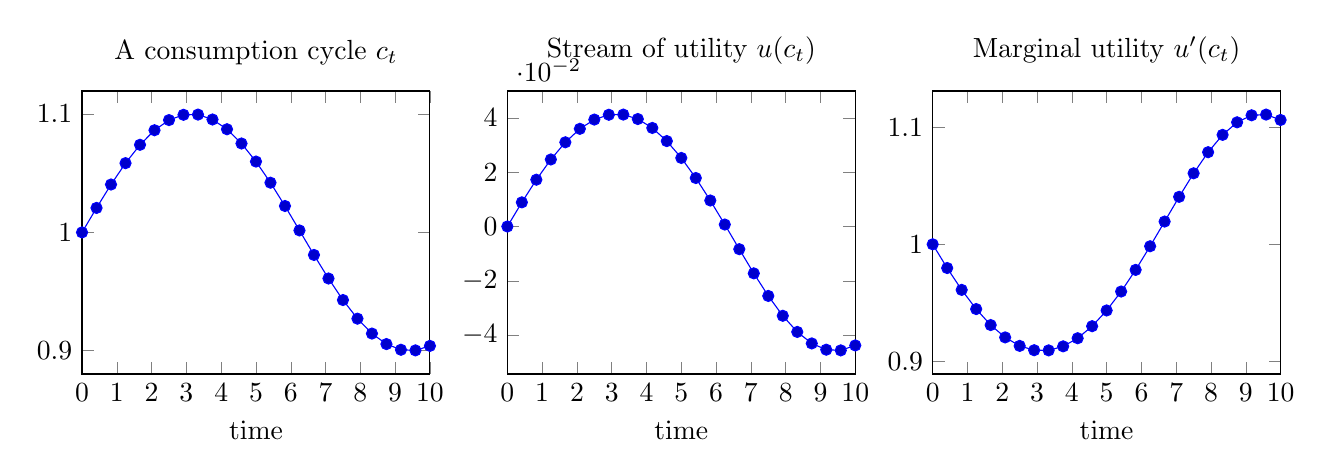
\begin{tikzpicture}
 
	\begin{axis}[name=plot1,title=A consumption cycle $c_t$]
 
		\addplot {1+sin(deg(0.5*x))/10};
 
    	\end{axis}
 
 
	\begin{axis}[name=plot2,at=(plot1.right of south east), anchor=left of south west,title=Stream of utility $u(c_t)$]
 
		\addplot {log10(1+sin(deg(0.5*x))/10)};
 
    	\end{axis}

 
	\begin{axis}[name=plot3,at=(plot2.right of south east), anchor=left of south west,,title=Marginal utility $u'(c_t)$]
 
		\addplot {1/(1+sin(deg(0.5*x))/10)};
 
    	\end{axis}
  
\end{tikzpicture}
\end{document}